% % APÊNDICES--------------------------------------------------------------------

\begin{apendicesenv}
% \partapendices

% % Primeiro apêndice------------------------------------------------------------
\chapter{COMPUTER INSTRUCTOR - PROTOTIPAGEM MOBILE}
\label{chap:apendiceA}


\begin{figure}[H]
    \centering
    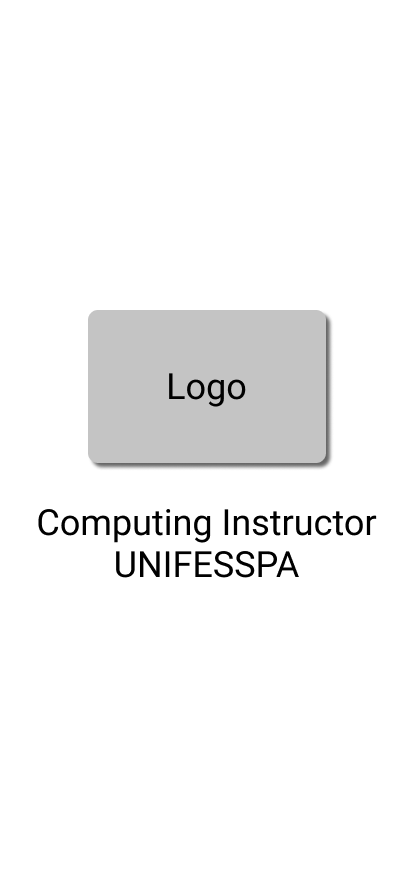
\includegraphics[width=0.5\textwidth]{figuras/Apêndice A/Splash creen.png}
\end{figure}


\begin{figure}[H]
    \centering
    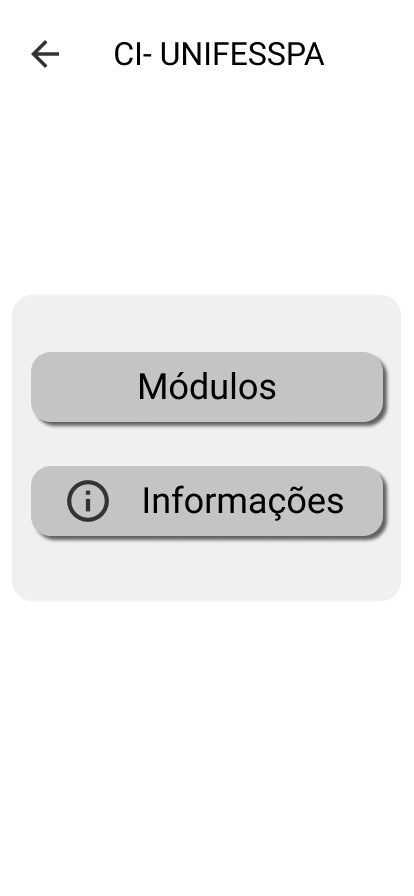
\includegraphics[width=0.5\textwidth]{figuras/Apêndice A/Presentation.png}
\end{figure}

\begin{figure}[H]
    \centering
    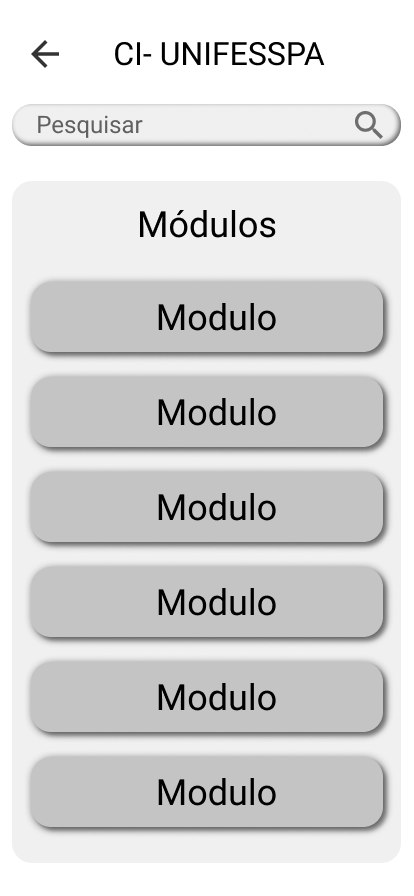
\includegraphics[width=0.5\textwidth]{figuras/Apêndice A/Module.png}
\end{figure}

\begin{figure}[H]
    \centering
    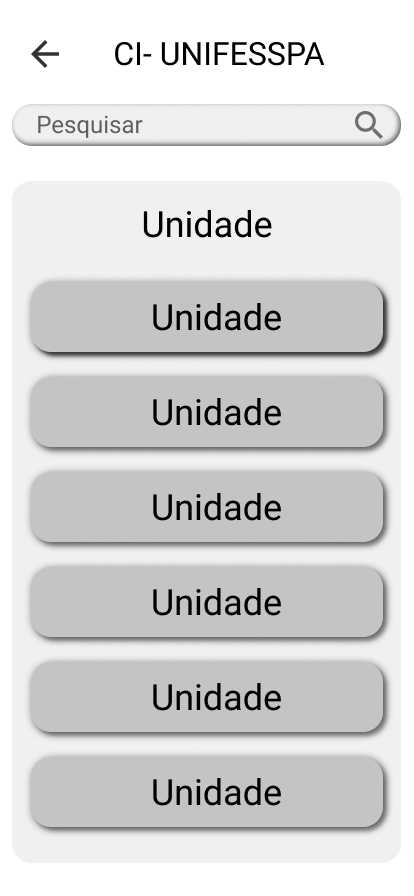
\includegraphics[width=0.5\textwidth]{figuras/Apêndice A/Unity-module.png}
\end{figure}

\begin{figure}[H]
    \centering
    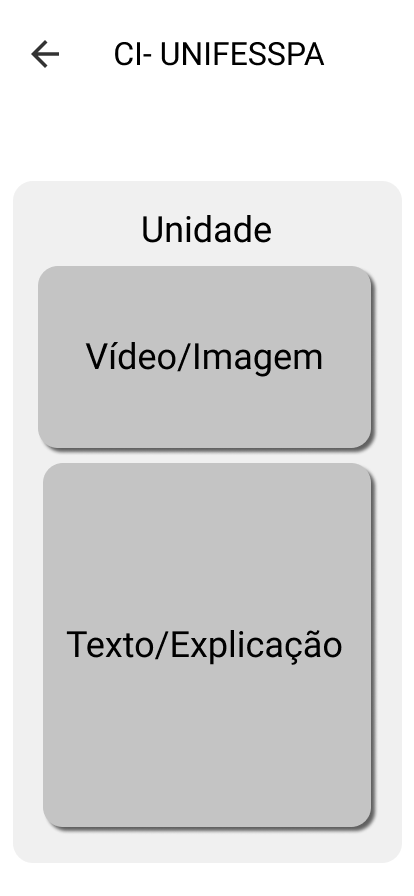
\includegraphics[width=0.5\textwidth]{figuras/Apêndice A/Unity-info.png}
\end{figure}

\begin{figure}[H]
    \centering
    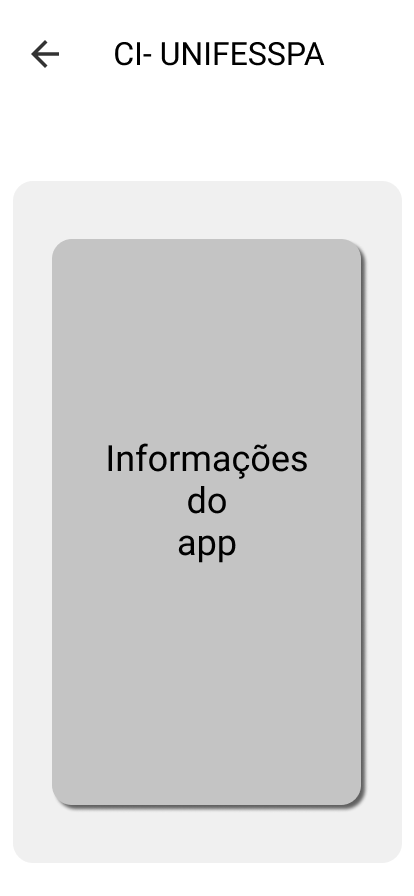
\includegraphics[width=0.5\textwidth]{figuras/Apêndice A/Info.png}
\end{figure}

% 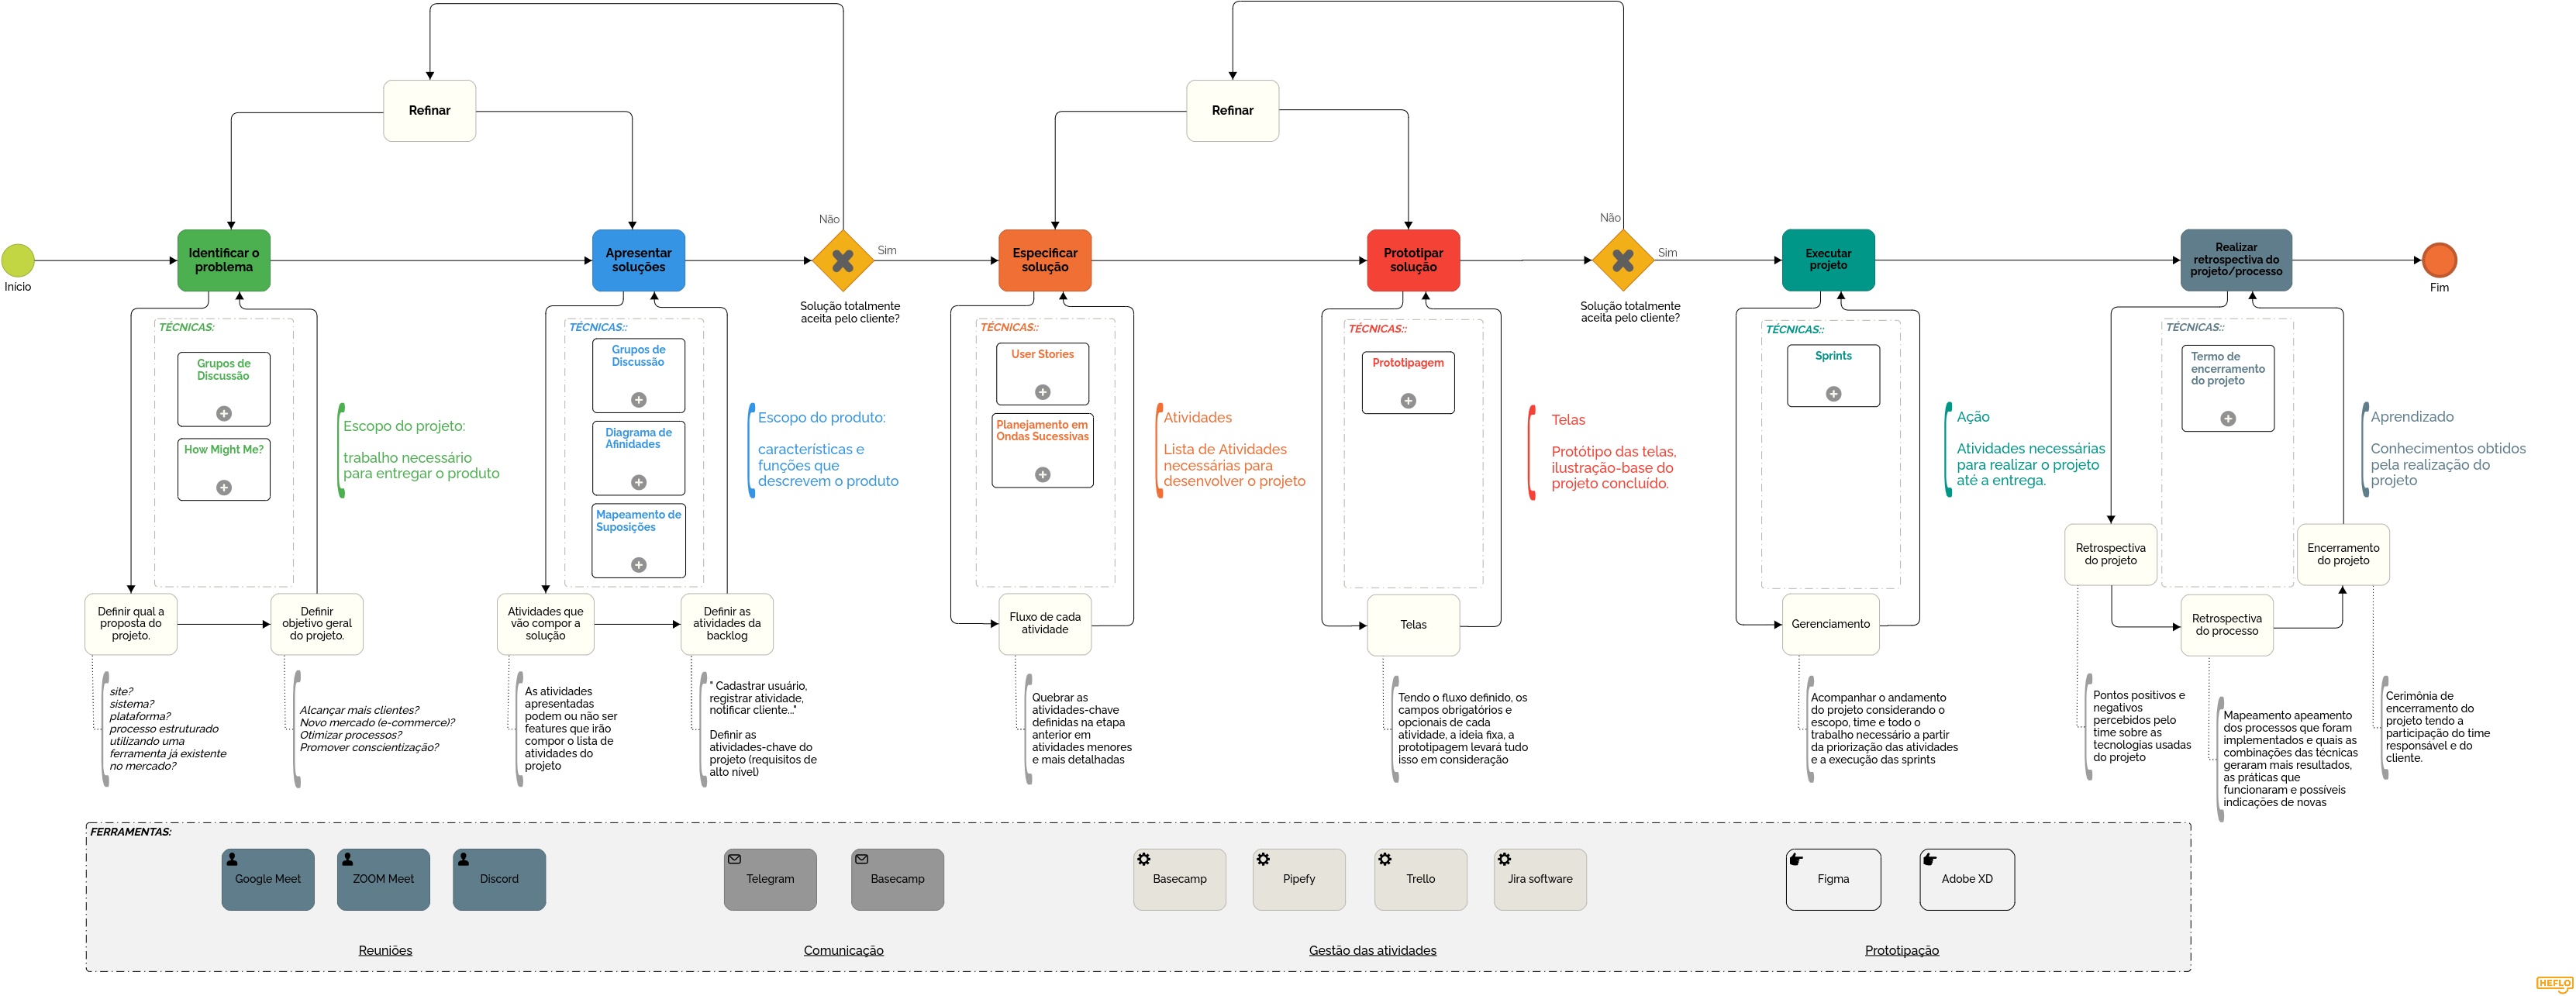
\includepdf[pages=-]{03-pos-textuais/apendices/estrutura.pdf}

% \chapter{Formulário diagnóstico}
% \label{chap:formulario}

% 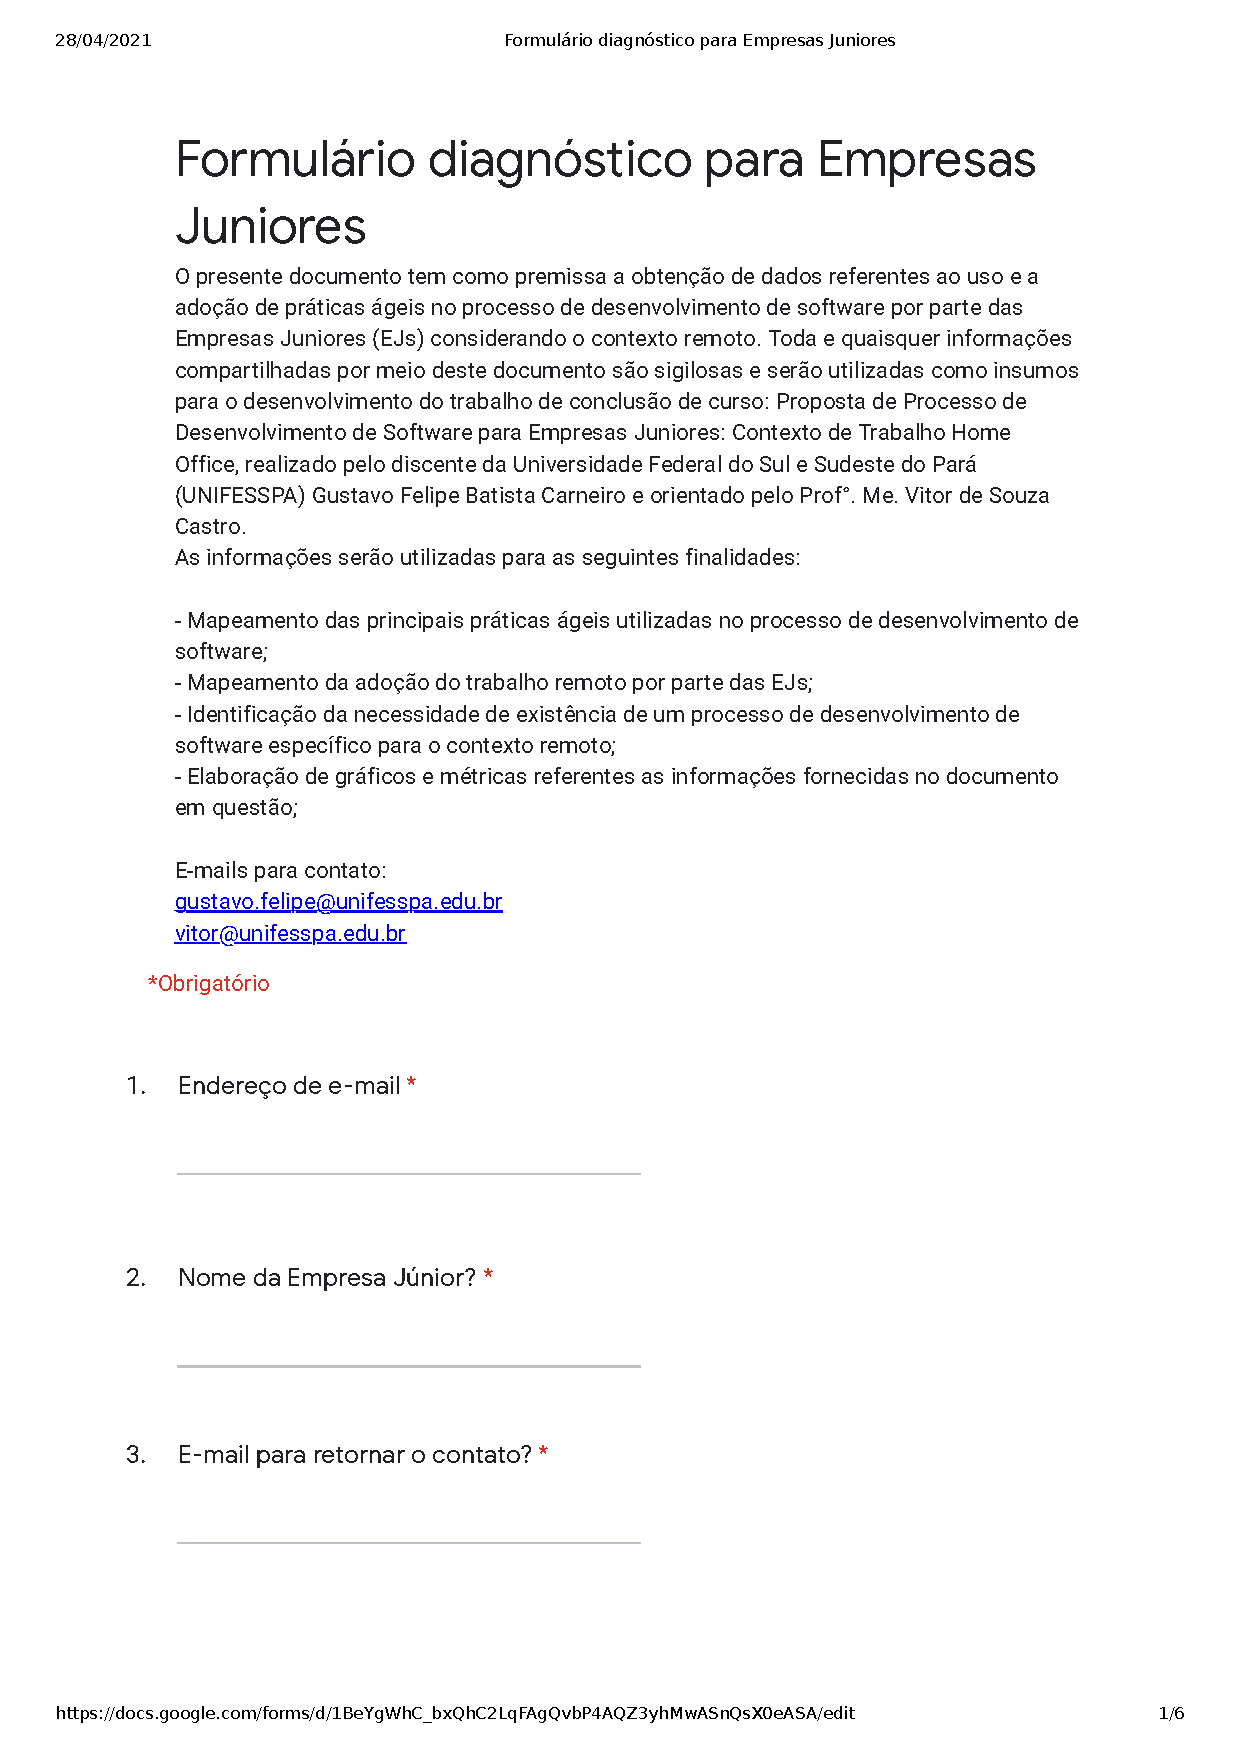
\includepdf[pages=-]{03-pos-textuais/apendices/formulario.pdf}


% \includepdf[pages=-]{03-pos-textuais/apendices/fomulario.pdf}
% 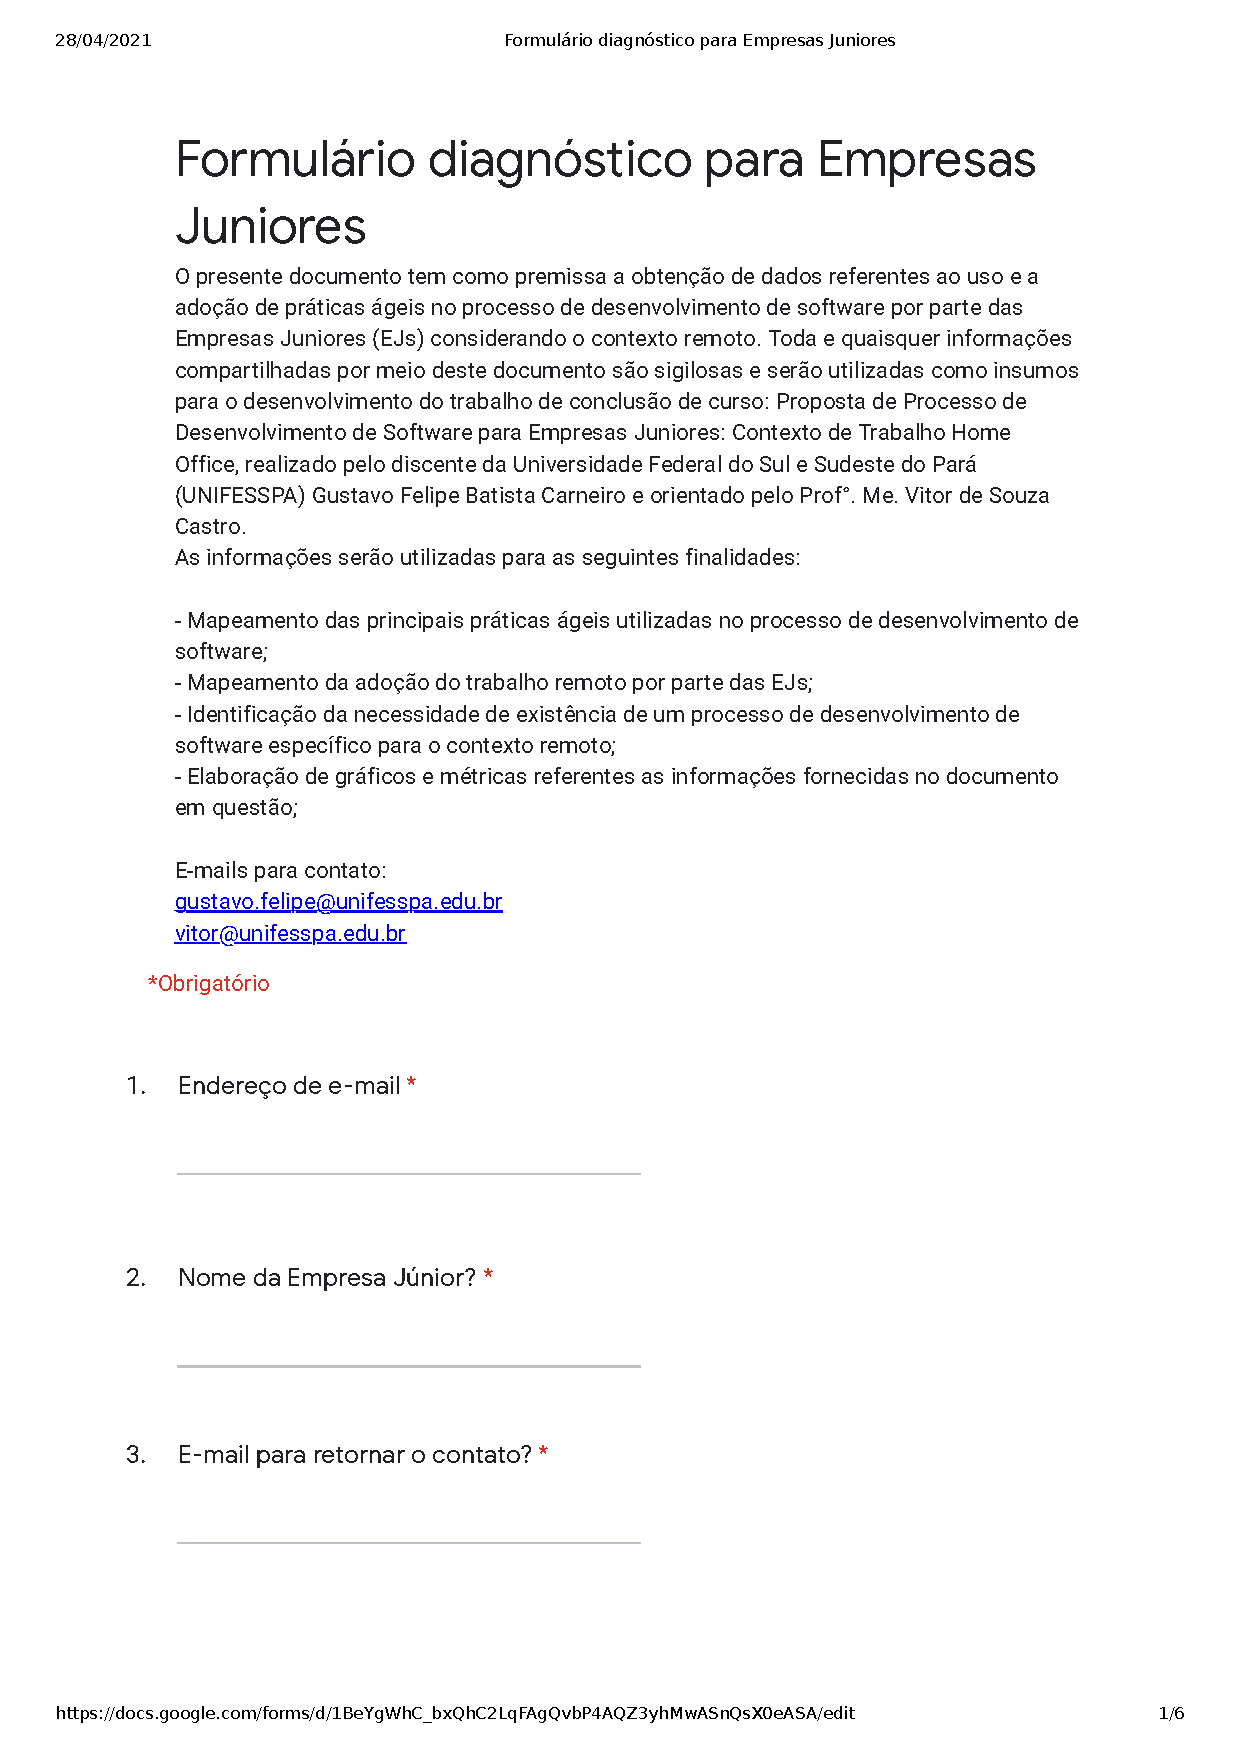
\includegraphics{03-pos-textuais/apendices/formulario.pdf}
% Lembre-se que a diferença entre apêndice e anexo diz respeito à autoria do texto e/ou material ali colocado.

% Caso o material ou texto suplementar ou complementar seja de sua autoria, então ele deverá ser colocado como um apêndice. Porém, caso a autoria seja de terceiros, então o material ou texto deverá ser colocado como anexo.

% Caso seja conveniente, podem ser criados outros apêndices para o seu trabalho acadêmico. Basta recortar e colar este trecho neste mesmo documento. Lembre-se de alterar o "label"{} do apêndice.

% Não é aconselhável colocar tudo que é complementar em um único apêndice. Organize os apêndices de modo que, em cada um deles, haja um único tipo de conteúdo. Isso facilita a leitura e compreensão para o leitor do trabalho.

% % Novo apêndice----------------------------------------------------------------
% \chapter{Nome do outro apêndice}
% \label{chap:apendiceB}

% conteúdo do novo apêndice
\chapter{COMPUTER INSTRUCTOR - PROTOTIPAGEM WEB}
\label{chap:apendiceB}


\end{apendicesenv}


